\chapter{Progettazione Concettuale}

\section{Premesse alla lettura dei diagrammi}

\subsection{Modelli Utilizzati}

Procediamo alla modellizzazione del mini-mondo, partendo dalla progettazione concettuale.

Questa fase di progettazione è stata svolta utilizzando, oltre che il modello \textbf{UML} nella forma di un \textbf{Class Diagram}, anche il modello \textbf{EER}, ovvero \textbf{Enhanced Entity Relationship}, per cogliere meglio aspetti del dominio che un modello \textbf{ER} classico non avrebbe potuto cogliere, come ad esempio \textbf{generalizzazioni e specializzazioni}.

\subsection{Precisazioni sui Diagrammi}

\subsubsection{EER Diagram}

Vista la densità del diagramma \textbf{EER}, si è deciso d'introdurre un \textbf{color coding} per facilitarne la lettura:

\begin{itemize}
  \item \textcolor{PRIMARY}{Entità}, e dunque Specializzazioni in \textcolor{PRIMARY}{arancione};
  \item \textcolor{CONTRAST}{Relazioni} in \textcolor{CONTRAST}{celeste};
  \item \textcolor{NEWGREEN}{Attributi} in \textcolor{NEWGREEN}{verde};
\end{itemize}

Inoltre, in caso di accavallamento di linee, si è deciso d'interrompere la linea in secondo piano in corrispondenza di un intersezione, così da evidenziare i diversi collegamenti.

\subsubsection{UML Class Diagram}

Per migliorare la leggibilità dei diagrammi, si è deciso di specificare le \textbf{molteplicità} degli attributi esclusivamente per sottolineare la possibilità di essere valorizzato a \textbf{NULL}. 

In tali casi si è utilizzata la molteplicità \textbf{[\(0..1\)]} esclusivamente per gli attributi di tipo \textbf{Bool}, mentre \textbf{[\(0..*\)]} per gli altri.

\bigskip

\begin{note}[Leggibilità dei Diagrammi]
  In caso di problemi di leggibilità dei diagrammi, sono disponibili le versioni originali nella pagina GitHub del progetto: \href{https://github.com/RiccardoElena/UninaDelivery/blob/develop/db/docs/sources/ER_Diagram.pdf}{\textit{\underline{ER Diagram}}} e \href{https://github.com/RiccardoElena/UninaDelivery/blob/develop/db/docs/sources/UML_Class_Diagram.pdf}{\textit{\underline{UML Class Diagram}}}.
\end{note}

\newpage
% TODO for EER diagram @zGenny:
% [x]: add assosation class with Date field to drives association
% [x]: to fix the "not world wide standard of zipcode problem" we can use both zipcode and country as primary key for the zone entity
% [x]: add Price field to the Shipping entity as a calculated field. It will after removed in the restructuring phase
% [x]: add the "isAvailable" field to the Driver entity
% [x]: change the "OnTravel" field to "isAvailable" to the Vehicle entity for more felxibility
% [x]: chenge the "IsCompleted" field to the Order entity to a calculated field. It can been extracted checking if all products in the order are in a shipment to the order maker. This one is gonna be stored in the restructured
% FIXME: @RiccardoElena hope we dont consider IsCompleted when there are no products in the order or we wont be able to have an history of the orders.
% [x]: add "HasArrived" field to the Shipment entity, to check if the shipment went to the destination or not
% [x]: remove $FiscalCode" field to the Account entity, it's not needed
% [x]: in the end export the new diagram as a pdf and replace the old one
\section{Enhanced Entity Relationship Diagram}
\begin{center}
  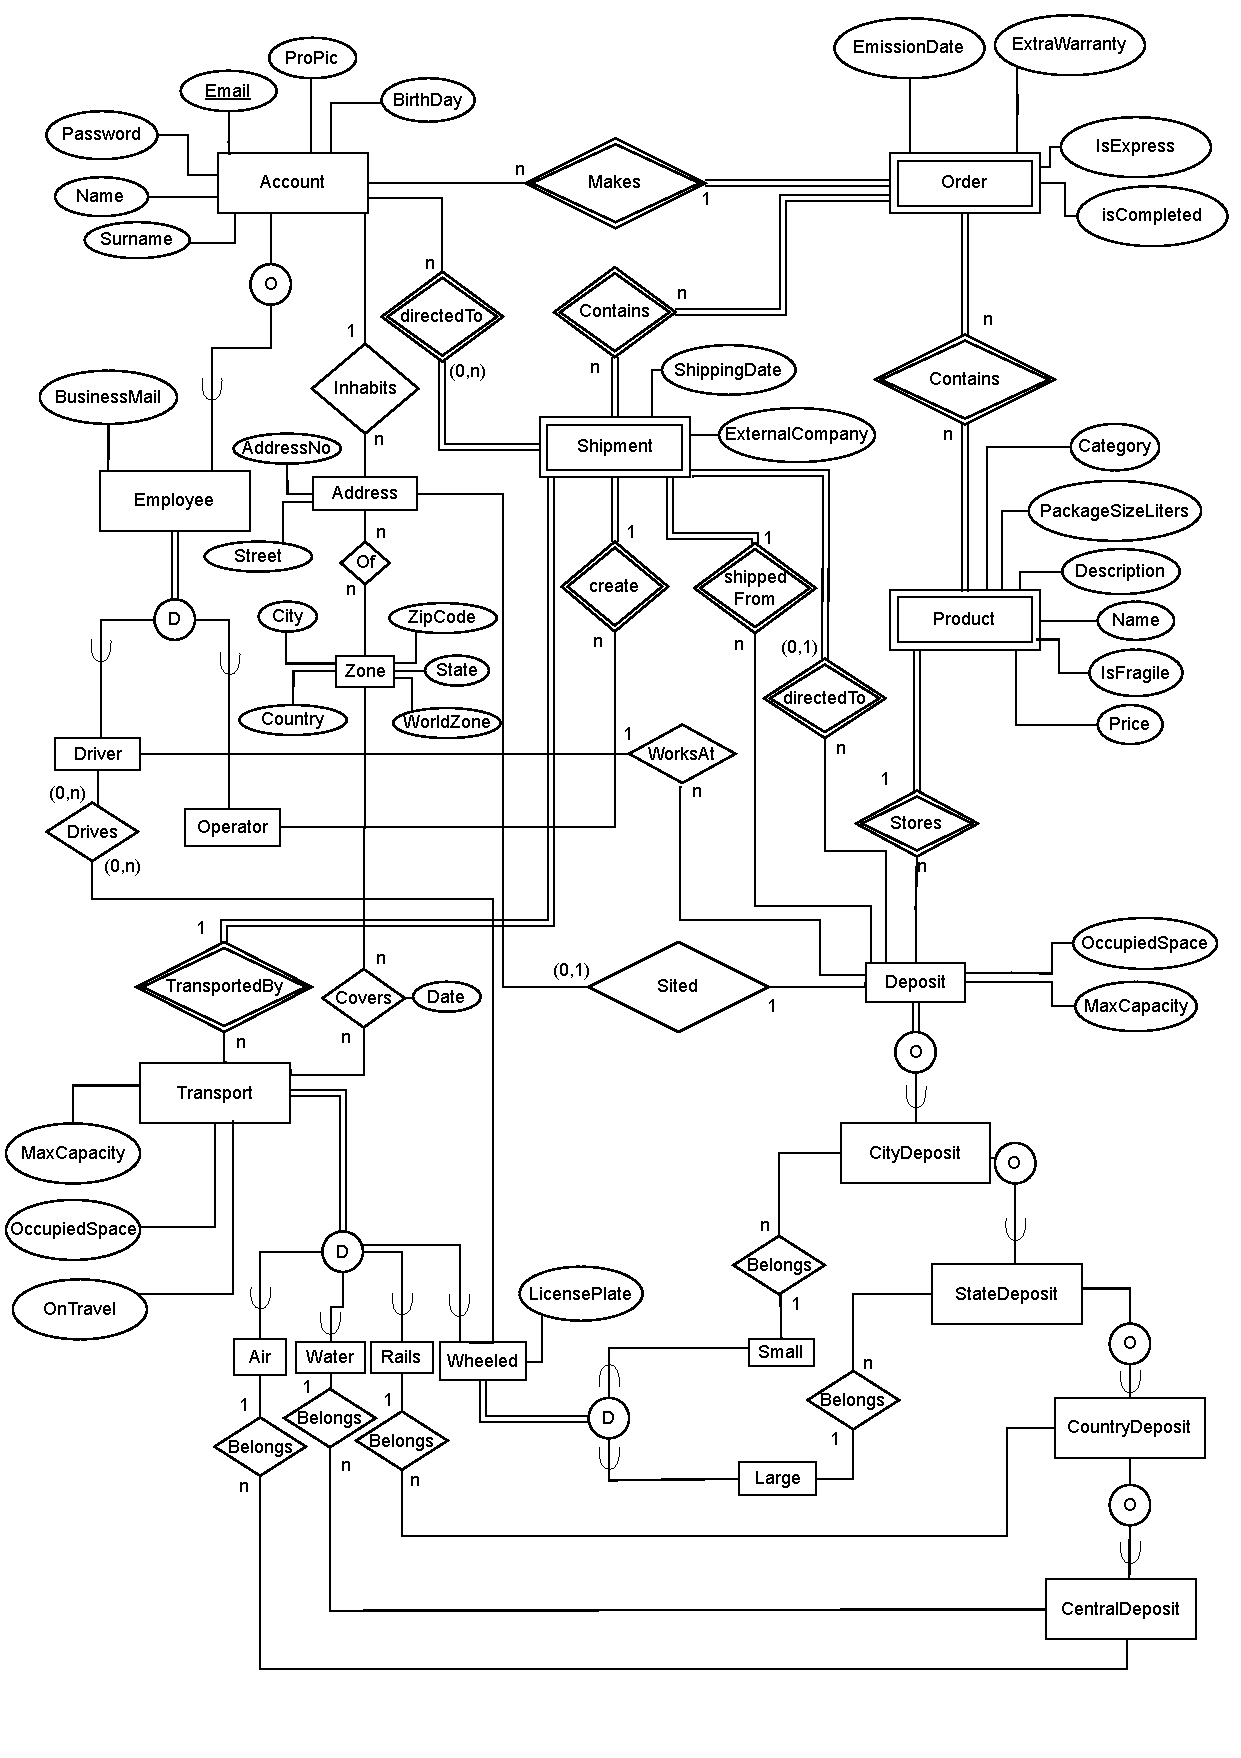
\includegraphics[width=0.9\textwidth]{ER_Diagram.pdf}
\end{center}

% TODO: need to re-export the UML diagram with the new changes. All the changes in the ER diagram are already done in the UML diagram

\section{UML Class Diagram}
\begin{center}
  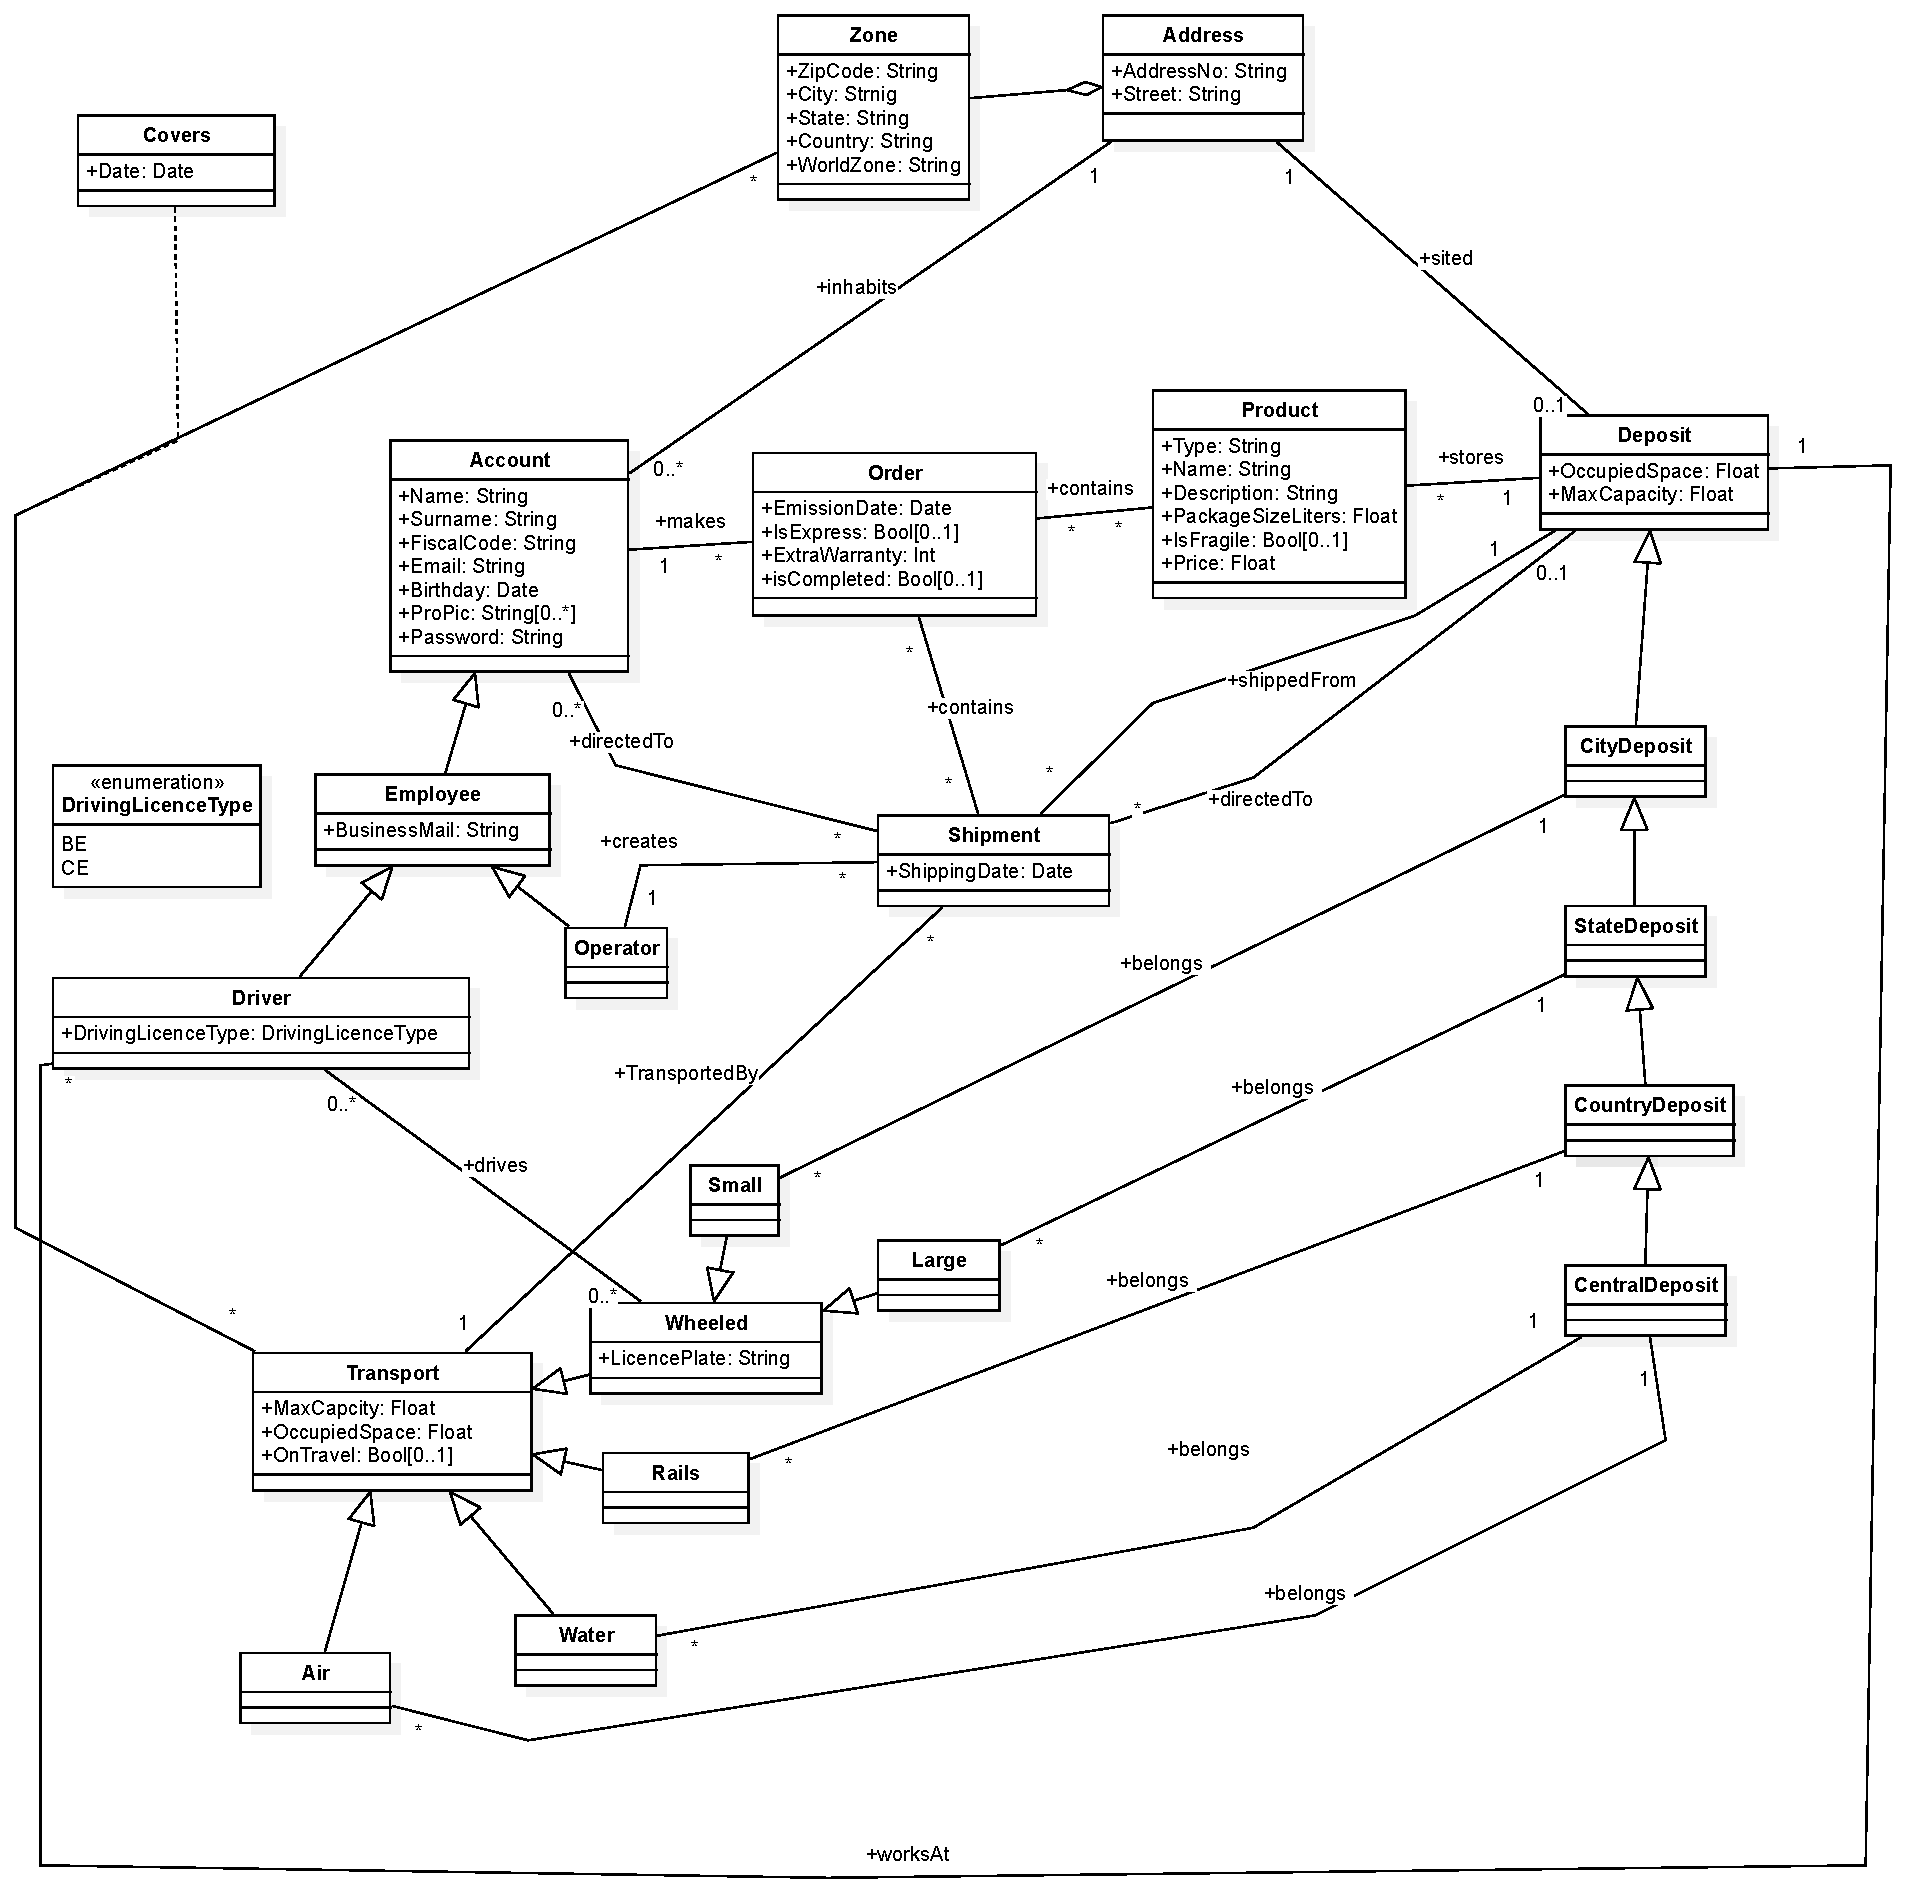
\includegraphics[width=\textwidth]{UML_Class_Diagram.pdf}
\end{center}

\newpage

\section{Ristrutturazione del Diagramma UML}

\subsection{Considerazioni sulla Ristrutturazione}

\subsubsection{Attributi Multipli e Multivalore}

Nello schema concettuale non sono presenti attributi \textbf{Multipli} o \textbf{Multivalore}, in quanto non sono stati ritenuti necessari per la rappresentazione del mini-mondo.

\subsubsection{Attributi Derivati}

Nello schema concettuale sono presenti due attributi \textbf{Derivati}:

\begin{itemize}
  \item L'attributo \textbf{Price} dell'entità \textbf{Shipment}, il quale però non ha necessità di essere conservato, non essendo un attributo di frequente richiesta per il sistema richiesto, e che quindi può essere eventualmente calcolato \textit{on-the-fly} in fase d'interrogazione del database basandosi sugli indirizzi di partenza e arrivo della spedizione e sulle eventuali modalità extra di consegna specificate in \textbf{Order}, come \textit{ExtraWarranty} e \textit{IsExpress}.
  \item L'attributo \textbf{IsCompleted} dell'entità \textbf{Order}, invece, si è scelto di conservarlo, in quanto è un attributo che può essere richiesto frequentemente dal sistema, e richiede un controllo relativamente complesso per essere valorizzato. Sarebbe necessario infatti controllare che tutti i prodotti dell'ordine siano stati spediti al destinatario, e che tali spedizioni siano andate a buon fine, coinvolgendo ben quattro entità: \textbf{Order}, \textbf{Product}, \textbf{Shipment} e \textbf{Account}. % * We should add a trigger that does this the first time
\end{itemize}

\subsubsection{Generalizzazioni e Specializzazioni}

Le varie \textbf{Generalizzazioni} e \textbf{Specializzazioni} presenti nello schema concettuale sono state ristrutturate usando metodologie diverse, in base alla loro natura.

\begin{itemize}
  \item[\textbf{Employee}] Essendo la specializzazione \textbf{Totale Disgiunta}, ed essendo le classi coinvolte in poche associazioni, si è scelto di accorpare la classe generale in quelle specializzate.
  \item[\textbf{Account}] Essendo la specializzazione \textbf{Parziale Overlapping}, si è deciso di trasformarla in \textbf{Associazione}, limitando così il più possibile il numero di campi \textbf{NULL} e di \textbf{Vincoli d'Integrità}.
  \item[\textbf{Deposit}] In questo caso trattandosi di una gerarchia di specializzazione si è scelto di accorpare a cascata le classi specializzate in quella generale, non avendo le classi specializzate attributi ed essendo tutte coinvolte in un'unica associazione concettualmente identica che verrà successivamente analizzata.
  \item[\textbf{Transport}] Analogamente a quanto visto per \textbf{Deposit}, nonostante non si tratti di una gerarchia, si è scelto di accorpare le classi specializzate in quella generale. 
\end{itemize}

\subsubsection{Analisi delle Ridondanze}

Vediamo infine le ridondanze presenti nello schema concettuale, e come sono state rimosse.

Dalla ristrutturazione delle \textbf{Specializzazioni} di \textbf{Transport} sono emersi quattro attributi che servono essenzialmente lo stesso scopo ma per tipologie diverse di mezzi di trasporto: \textbf{Licence Plate}, \textbf{TrainNo}, \textbf{IMOCode} e \textbf{FlightNo}. Si è quindi deciso di accorpare questi attributi in un unico attributo \textbf{TransportID}, che può essere valorizzato con un identificativo univoco condiviso tra le tipologie di mezzi di trasporto, eliminando la possibilità di valori \textbf{NULL} o di valori uguali per tipi di mezzi diversi che imponevano aggiunta di vincoli o presenza di più attributi.

Inoltre la ristrutturazione delle \textbf{Specializzazioni} di \textbf{Deposit} ha fatto emergere quattro associazioni identiche a meno di vincoli che le riguardano, ovvero le associazioni \textbf{belongs}. È possibile dunque ridurle ad un'unica associazione preservando i vincoli.

In ultima analisi, la classe \textbf{Shipment} è coinvolta in due associazioni sematnicamente identiche, che si distinguoni solo per molteplicità e seconda classe coinvolta, ovvero \textbf{Account} e \textbf{Deposit}. In particolare quella con \textbf{Account} è un'associazione circolare, essnedo entrambe le classi associate anche con \textbf{Order}. Si è quindi deciso di eliminare l'associazione con \textbf{Account}, essendo il destinatario della spedizione già noto tramite \textbf{Order}.

\subsection{Class Diagram Ristrutturato}

% TODO: @zGenny review restructured diagram, if it's ok export it and uncommend this part

% \begin{center}
  % ! USE THE NAME MENTIONED HERE FOR THE FILE
%   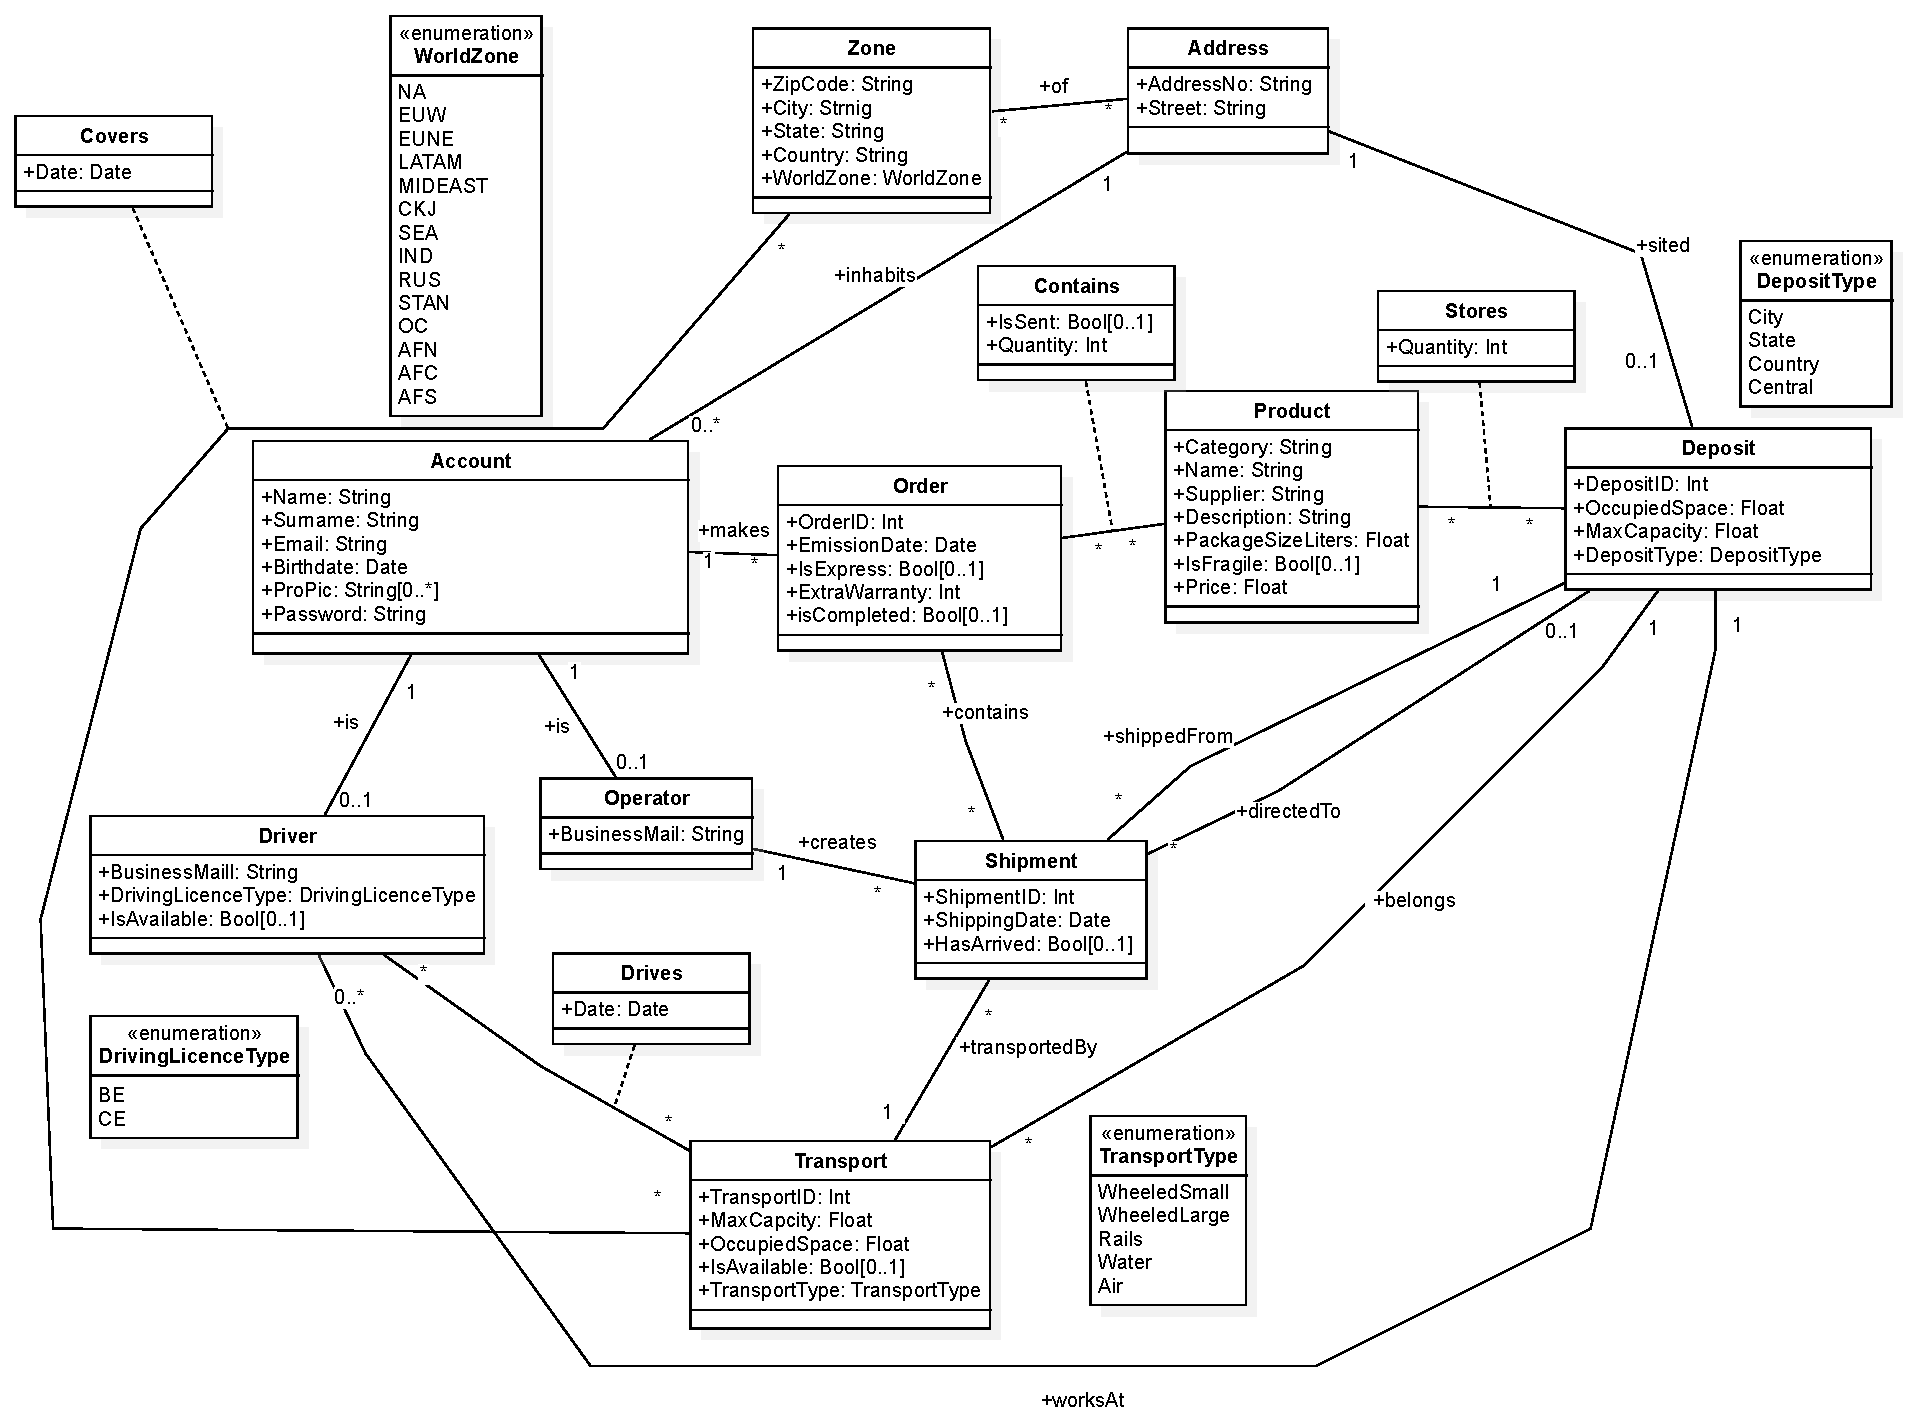
\includegraphics[width=\textwidth]{UML_Class_Diagram_Restructured.pdf} 
% \end{center}

\newpage

\section{Dizionari}

\subsection{Dizionario delle Classi}

\customTable{YYY}[Dizionario delle classi]{Classe & Descrizione & Attributi}{
  Account & Generico account che utilizza il sistema per effettuare ordini & \textbf{Name:} Nome dell'utente \newline \textbf{Surname}: Cognome dell'utente \newline \textbf{FiscalCode}: Codice fiscale utente \\
  Valore 4 & Valore 5 & Valore 6 \\
}
  




% TODO: @RiccardoElena @zGenny write this section
  % it should contains:
  % [x] all the considerations about the UML diagram
  % [x] the changes made to the UML diagram
  % [ ] the new UML diagram
  % [ ] constrints dictonary (table (?)). Styled as the example in the slides